\documentclass{ctexart}
\usepackage[utf8]{inputenc}
\usepackage{tikz}
\usetikzlibrary{positioning, shapes.geometric}
\usepackage{tikz}
\usetikzlibrary{calc,positioning}
\usepackage{graphics}
\usepackage{graphicx}
\usepackage{float}
\usepackage{subfig}
%\usepackage{subfigure}
\usepackage{subfloat}
\usepackage{url}
\graphicspath{{img/}}
\title{\vspace{-2.5cm}Julia集的分析和探索}
\author{顾格非\\3210103528}

\begin{document}

\maketitle
\begin{abstract}
    Julia set是一个在复平面上形成分形的点的集合\cite{a1}。以法国数学家加斯顿·朱利亚(Gaston Julia)的名字命名。本文回顾了相关的数学理论,设计了相关算法与代码实现,并展示通过代码得到的数值算例并进行了分析,最后分析了Julia集合与Mandelbrot集合的关系并得出结论。
\end{abstract}
\section{引言}

Julia集合以法国数学家加斯顿·茱莉亚(Gaston Julia)的名字命名,他于1915年调查了它们的性质,并在1918年发表了著名的论文:Mémoire sur l'itération des fonctions rationnelles。

1979年,在计算机的帮助下,B. B. Mandelbrot研究了Julia集合,并试图对所有可能的形状进行分类,并提出了Mandelbrot集合。
\vspace{-0.3cm}
\section{数学理论}
\vspace{-0.3cm}
\subsection{定义}
Julia集合可由$f_c(z)=z^2+c$反复迭代得到,对于固定的复数c,取某一$z$值(如$z=z_0$),可以得到序列:
$$
z_0,f_c(z),f_c(f_c(z)),f_c(f_c(f_c(z))),……
$$

这一序列可能发散于无穷大或始终处于某一范围之内并收敛于某一值。我们将使其不扩散的z值的集合称为Julia集合。

\subsection{Julia集的不变性和对称性}
如果 c 是实数,则 Julia 集围绕实轴镜像。具有非零虚部的其他 c 值具有 180 度旋转对称性\cite{a2}。

Julia 集的点对于 $f(z)$ 的进一步迭代是“不变的”。这里,不变性并不意味着 $f(z_j )=z_j$,而是对于属于集合$J$的任何点$z_j$ ,$f(z_j)$ 也是$J$的成员。

\subsection{逃逸准则}
对于一个复数$z_{n}=x_{n}+iy_{n}$,定义模$\left|z_{n}\right|=\sqrt{x_{n}^{2}+y_{n}^{2}}$。则如果对于一个复数序列$\{z_1, z_2 \ldots z_n\}$有$\left|z_{j}\right|>\max (2,|c|)$,则序列将逃逸到无穷大。

为了确定每个$z$是否属于M集,借助上面的逃逸准则,若某一次迭代后$\left|z\right|>2$,我们立即就判定为不在集合内,这样可以方便的用计算机实现。

\section{算法}
设定一个迭代次数的上限$N$ ,当经过 $N$次迭代,$f_c(z)$仍然没有超过 2,我们就认为这个点就属于Julia集合 (尽管一些点也可能混入Julia集合);否则,就说明该点不Julia集合在中,并记录这个点挑出循环时的次数。这样平面上每个点都对应了一个循环次数$i$(对于集合内的点,$i=N$;对于集合外的点,$i<N$),然后将$i$映射到颜色上去进行着色。
\begin{center}
\begin{tikzpicture}[node distance=10pt]
  \node[draw, rounded corners]                        (start)   {输入某个复数c};
  \node[draw, below=of start,align=center]                         (step 1)  {遍历所有的复数$z_0$ \\ 循环计数器i=1};
  \node[draw, below=of step 1,align=center]                        (step 2)  {$z=z^2+c$\\i=i+1};
  \node[draw, diamond, aspect=2, below=of step 2,align=center]     (choice)  {$z<2?$\\$i\leq N?$ };
  
  \node[draw, rounded corners, below=of choice]  (end)    {记录挑出循环的i};
  \node[draw, rounded corners, below=of end]  (end2)     {根据i的大小映射到不同的颜色};
  
  \draw[->] (start)  -- (step 1);
  \draw[->] (step 1) -- (step 2);
  \draw[->] (step 2) -- (choice);
  \draw[->] (choice) -- node[left]  {No} (end);
  \draw[->] (choice.east)--($(choice.east)+(1,0)$) --node[left]{Yes}  ($(step 2.east)+(1.88,0)$) -- (step 2.east);
  \draw[->] (end) -- (end2);
\end{tikzpicture}
\end{center}


\section{数值算例及分析}
下面两个图分别取c为实数和复数的情况,分别展现了Julia集合的反射对称性和旋转对称性。
\begin{figure}[h]
	\centering
	\begin{minipage}{0.4\linewidth}
		\centering
		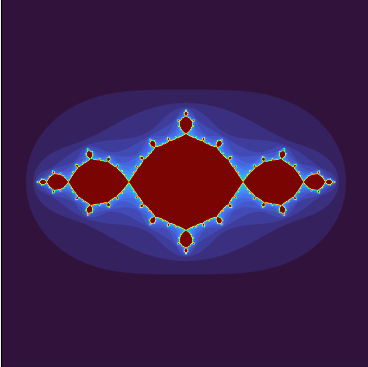
\includegraphics[width=0.55\linewidth]{-1.png}
		\caption{$c=-1$}% 标题
		\label{chutian1}%文中引用该图片代号
	\end{minipage}
	%\qquad 这行代码用来换行的!
	\begin{minipage}{0.4\linewidth}
		\centering
		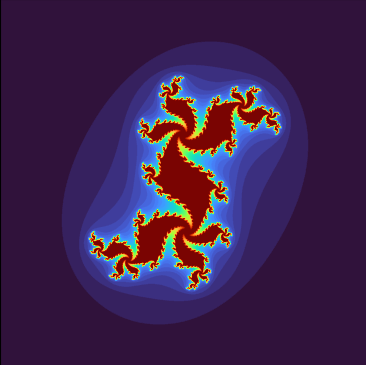
\includegraphics[width=0.55\linewidth]{0.3_0.6.png}
		\caption{$c=0.3+0.6i$}
		\label{chutian2}%文中引用该图片代号
	\end{minipage}
\end{figure}

以下展现了一个迭代的过程。通过控制最大迭代次数$N$的增大,图形精度越来越高,红色的面积越来越小。

\begin{figure}[H]
	\centering
	\subfloat[N=5]{
	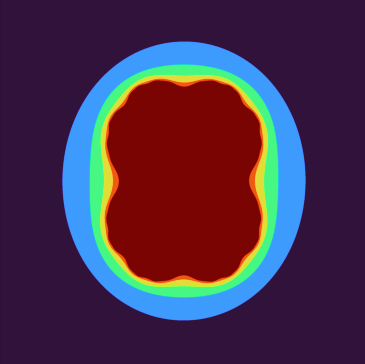
\includegraphics[width=2cm]{5.png}
	}
	\subfloat[N=15]{
	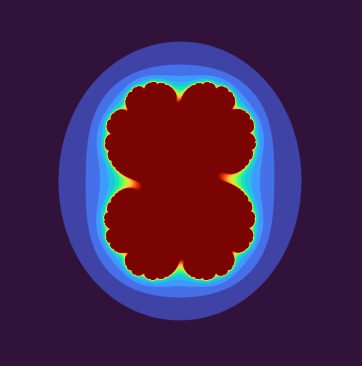
\includegraphics[width=2cm]{15.png}
	}
	\subfloat[N=100]{
	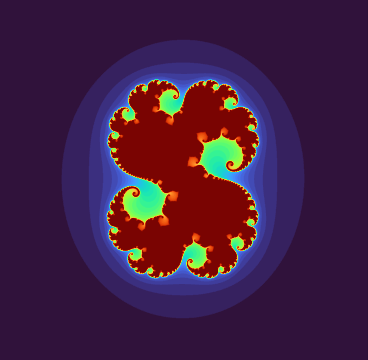
\includegraphics[width=2cm]{0.273_0.007.png}
	}
	\subfloat[N=500]{
	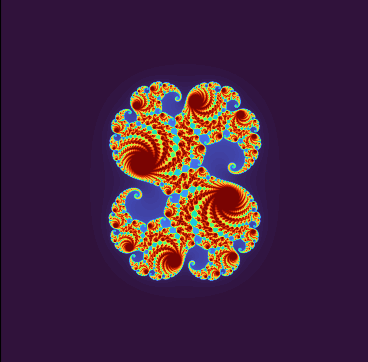
\includegraphics[width=2cm]{500.png}
	}
	\caption{不同迭代次数下$c=0.273+0.007i$的图像}
\end{figure}
本文前面所讨论的迭代方程都是基于$z=z^2+c$,但事实上,Julia本人还研究过诸如$z=z^{4}+\frac{z^{3}}{z-1}+\frac{z^{2}}{z^{3}+4 z^{2}+5}+c$的迭代方程,以下是我改变迭代方程的算例展示:
\begin{figure}[H]
	\centering
	\subfloat[$z=z^2+c$]{
	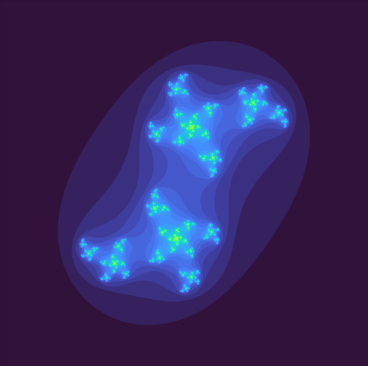
\includegraphics[width=3cm]{2.png}
	}
	\subfloat[$z=z^3+c$]{
	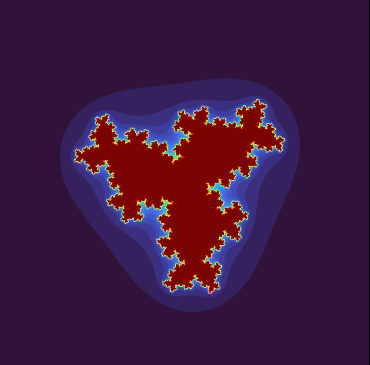
\includegraphics[width=3cm]{3.png}
	}
	\subfloat[$z=z^4+c$]{
	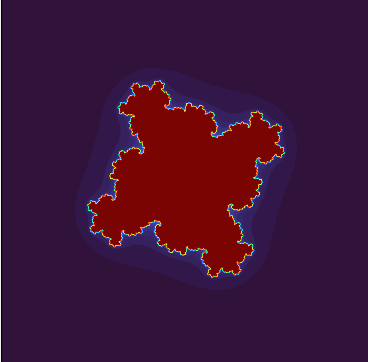
\includegraphics[width=3cm]{4.png}
	}
	\caption{不同迭代方程下$c=0.273+0.7i$的图像}
\end{figure}
\section{与mandelbrot的关系}
众所周知的 Mandelbrot 集形成了 Julia 集的一种索引。一个 Julia 集要么是连通的,要么是不连通的,从 Mandelbrot 集合内选择的 c 值是连通的,而从 Mandelbrot 集合外部选择的 c 值是不连通的。不连贯的集合通常被称为“dust”,无论以何种分辨率查看它们,它们都由单个点组成。

\begin{figure}[h]
\centering
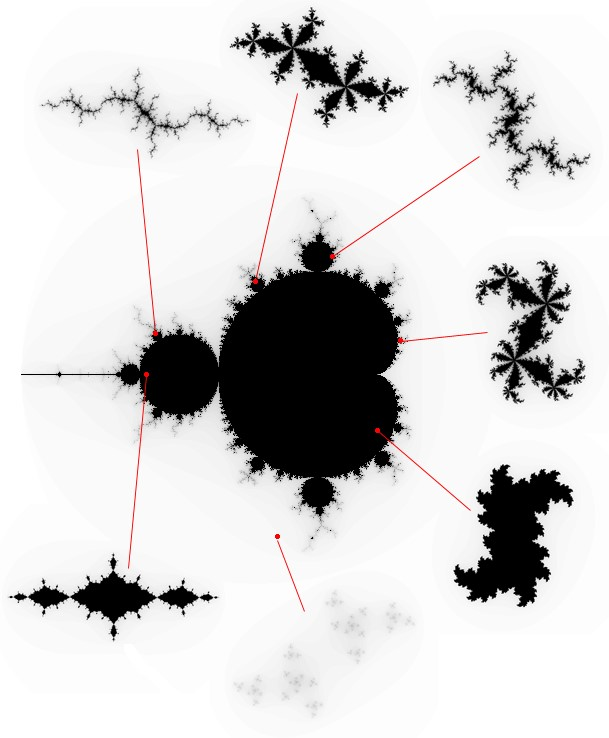
\includegraphics[width=0.4\linewidth]{julia_mandel.jpg}
\caption{mandelbrot与Julia连通性可视化}
\label{fig:output2}
\end{figure}
\section{结论}
Julia集合波谲云诡的数学形态展现了数学世界的奇妙,作为后人我深深感谢前人的工作和为数学的美所折服。

\bibliographystyle{plain}
\bibliography{ref}
\end{document}

